\chapter{Network Graphics And Animation}
\label{cha:graphics}

\section{Display strings}
\label{sec:ch-graphics:display-strings}

Display strings\index{display strings} specify the arrangement and
appearance of modules in graphical user interfaces (currently only
Tkenv): they control how the objects (compound modules, their
submodules and connections) are displayed. Display strings occur in
NED description's \fpar[ned!keywords!display]{@display}
property.

Display strings can be used in the following contexts:
\begin{itemize}
  \item \textit{submodules} -- display string may contain position, arrangement
        (for module vectors), icon, icon color, auxiliary icon, status text,
        communication range (as circle or filled circle), tooltip, etc.
  \item \textit{compound modules, networks} -- display string can specify
        background color, border color, border thickness,
        background image, scaling, grid, unit of measurement, etc.
  \item \textit{connections} -- display string can specify positioning, color,
        line thickness, line style, text and tooltip
  \item \textit{messages} -- display string can specify icon, icon color, etc.
\end{itemize}


\subsection{Display string syntax}

The display string syntax is a semicolon-separated list of tags.
Each tag consists of a key, an equal sign and a comma-separated list of
arguments:
\begin{verbatim}
@display("p=100,100;b=60,10,rect,blue,black,2")
\end{verbatim}

Tag arguments may be omitted both at the end and inside the
parameter list:
\begin{verbatim}
@display("p=100,100;b=,,rect,blue")
\end{verbatim}

\subsection{Display string placement}

The following NED sample shows where to place display strings in the code:

\begin{verbatim}
simple Queue
{
    parameters:
        @display("i=block/queue");
    ...
}

network SimpleQueue
{
    parameters:
        @display("bgi=maps/europe");
    submodules:
        sink: Sink {
            @display("p=273,101");
        }
        ...
    connections:
        source.out --> { @display("ls=red,3"); } --> queue.in++;
}
\end{verbatim}

\subsection{Display string inheritance}

Every module and channel object has one single display string object,
which controls its appearance in various contexts. The initial value of
this display string object comes from merging the \ttt{@display}
properties occurring at various places in NED files.
This section describes the rules \ttt{@display} properties are merged
to create the module or channel's display string.

\begin{itemize}
  \item Derived NED types inherit their display string from their base NED type.
  \item Submodules inherit their display string from their type.
  \item Connections inherit their display string from their channel type.
\end{itemize}

The base NED type's display string is merged into the current display string
using the following rules:

\begin{itemize}
  \item If a tag is present in the base display string, but not in the current one
        the whole tag (with all arguments) is added to the current display string.
        (e.g. base: \ttt{"i=icon,red"} current: \ttt{"p=2,4"} result: \ttt{"p=2,4;i=icon,red"})
  \item If a tag is present both in the base and in the current display string
        only tag arguments present in the base, but not in the current display string
        will be copied.
        (e.g. base: \ttt{"b=40,20"} current: \ttt{"b=,,oval"} result: \ttt{"b=40,20,oval"})
  \item If the current display string contains a tag argument with value "-" (hyphen)
        that argument is treated as empty and will not be inherited from other
        display strings. Requesting the value of this argument will return its the
        default value.
  \item If neither the base display string nor the current one has value for a tag
        a suitable default value will be returned and used.
\end{itemize}

Example of display string inheritance:
\begin{verbatim}
simple Base {
    @display("i=block/queue"); // use a queue icon in all instances
}
simple Derived extends Base {
    @display("i=,red,60");  // ==> "i=block/queue,red,60"
}
network SimpleQueue
{
    submodules:
        submod: Derived {
            @display("i=,yellow,-;p=273,101;r=70");  // ==> "i=block/queue,yellow;p=273,101;r=70"
        }
\end{verbatim}


\subsection{Display string tags used in submodule context}

The following tags define how a module appears on the Tkenv user interface
if it is used as a submodule:
\begin{itemize}
  \item{\ttt{b} -- shapes, colors}
  \item{\ttt{i} -- icon}
  \item{\ttt{is} -- icon size}
  \item{\ttt{i2} -- alternate (status) icon placed at the upper right corner of the main icon}
  \item{\ttt{p} -- positioning and layouting}
  \item{\ttt{r} -- range indicator}
  \item{\ttt{q} -- queue information text}
  \item{\ttt{t} -- text}
  \item{\ttt{tt} -- tooltip}
\end{itemize}

\subsubsection{Icons}
By default modules are represented by simple icons.
Using images for the modules is possible with the \ttt{i} tag.
See the \ttt{images} subfolder of your {\opp} installation for possible
icons. The stock images installed with {\opp} have several size variants.
Most of them have very small (vs), small (s), large (l) and
very large (vl) variants. You can specify which variant you want to use with
the \ttt{is} tag.
\begin{verbatim}
@display("i=block/source;is=l"); // a large source icon from the block icons group
\end{verbatim}

Sometimes you want to have similar icons for modules, but would like to
make them look a little different to create groups or to reflect status
information about the module. You can easily change the color of an already existing image.
The following example colorizes the \ttt{block/source} icon, 20\% red
\begin{verbatim}
@display("i=block/source,red,20")
\end{verbatim}

\begin{center}
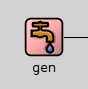
\includegraphics{figures/graphics-itag}
\end{center}

If you want to show state information about your module, you can use the \ttt{i2} tag to
add a small status icon to your main icon. This icon is displayed in the upper right corner
of your main icon. In most cases the \ttt{i2} tag is specified at runtime using
the \ffunc{setDisplayString()} method, so the icon can be changed dynamically based on the
module's internal state.
\begin{verbatim}
@display("i=block/queue;i2=status/busy")
\end{verbatim}

\begin{center}

\includegraphics{figures/graphics-i2tag}
\end{center}

\subsubsection{Shapes}
If you want to have simple, but resizable representation for your module, you can use
the \ttt{b} tag to create geometric shapes. Currently \ttt{oval} and \ttt{rectangle}
 is supported:
\begin{verbatim}
// an oval shape with 70x30 size, red background, black 4 pixel border
@display("b=70,30,oval,red,black,4")
\end{verbatim}

\begin{center}
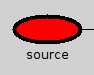
\includegraphics{figures/graphics-btag}
\end{center}

\subsubsection{Positioning, coordinates}

To define the position of a module inside an other one use the \ttt{p} tag.
If you do not specify a \ttt{p} tag for your module, the parent module will
automatically choose a position based on a layouting algorithm.
The following example will place the module at the given position:
\begin{verbatim}
@display("p=50,79");
\end{verbatim}

\begin{note}
The coordinates specified in the \ttt{p}, \ttt{b} or \ttt{r} tags are not necessarily
integers and measured in pixels. You can use the parent module's \ttt{bgs=$pix2unitratio$,$unit$} tag,
to set the scaling parameter and the unit of measurement for your module.
You can specify the ratio between 1 pixel and 1 unit with the \ttt{bgs} tag.
\end{note}

The \ttt{p} tag allows the automatic arrangement of module vectors. They can be
arranged in a row, a column, a matrix or a ring or you may specify their positions
later at runtime using the \ffunc{setDisplayString()} method. The rest of the arguments
in the \ttt{p} tag depends on the layout type:

\begin{itemize}
  \item \ttt{row -- p=100,100,r,$deltaX$} (A row of modules with $deltaX$ units between the modules)
  \item \ttt{column -- p=100,100,c,$deltaY$} (A column of modules with $deltaX$ units between the modules)
  \item \ttt{matrix -- p=100,100,m,$noOfCols$,$deltaX$,$deltaY$} (A matrix with $noOfCols$ columns.
            $deltaX$ and $deltaY$ units between rows and columns)
  \item \ttt{ring -- p=100,100,ri,$rx$,$ry$} (A ring (oval) with $rx$ and $ry$ as the horizontal and vertical radius.)
  \item \ttt{exact (default) -- p=100,100,x,$deltaX$,$deltaY$} (Place each module at $(100+deltaX, 100+deltaY)$.
            The coordinates are usually set at runtime.)
\end{itemize}

A matrix layout for a module vector:
\begin{verbatim}
@display("p=,,m,4,50,50");
\end{verbatim}

\begin{figure}[htbp]
  \begin{center}
    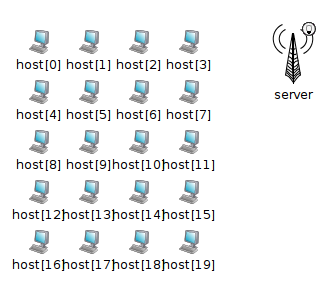
\includegraphics{figures/graphics-ptag}
    \caption{Matrix arrangement using the $p$ tag}
    \label{fig:graphics-ptag}
  \end{center}
\end{figure}

\subsubsection{Wireless range}
In wireless simulations it is very useful to show some kind of range
around your module. This can be an interference range, transmission range
etc. The following example will place the module at a given position,
and draw a 90 unit circle around it as a range indicator:
\begin{verbatim}
submodules:
    ap: AccessPoint {
        @display("p=50,79;r=90");
    }
\end{verbatim}

\begin{figure}[htbp]
  \begin{center}
    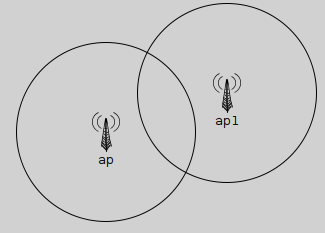
\includegraphics{figures/graphics-rtag}
    \caption{Range indicator using the $r$ tag}
    \label{fig:graphics-rtag}
  \end{center}
\end{figure}

\subsubsection{Additional decorations}
Sometimes you want to annotate your modules with additional information
to make your model more transparent. One special case is when you want to
show the length of a queue (\cclass{cQueue}) embedded somewhere in a module.
In the following example the Server simple module contains a \cclass{cQueue} object,
which was named by the \ffunc{queue.setName("procqueue")} method.
If we specify \ttt{q=procqueue} in the display string, Tkenv will descend into
the module (several levels deep if needed) and look for a queue object
named "procqueue". It will display the length of the queue object along the module.
\begin{verbatim}
@display("q=procqueue");
\end{verbatim}

\begin{center}
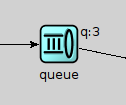
\includegraphics{figures/graphics-qtag}
\end{center}

You can add a text description to any module using the \ttt{t}
(displayed along the module) or \ttt{tt} tag (displayed as a tooltip).
The following example displays a short text along with the module
and adds a tooltip text too that can be seen by hovering over
them module with the mouse.

\begin{verbatim}
@display("t=Packets sent: 18;tt=Additional tooltip information");
\end{verbatim}

\begin{center}
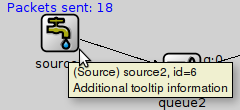
\includegraphics{figures/graphics-ttag}
\end{center}

\begin{note}
  Generally it makes no sense to assign static texts in the NED file. Usually the
  \ttt{t} and \ttt{tt} tags are used at runtime with the \ffunc{setDisplayString()}
  method.
\end{note}

To see detailed descripton of the display string tags check
Appendix \ref{cha:display-string-tags} about display string tags.

\subsection{Display string tags used in module background context}

The following tags describe what a module looks like if opened in
Tkenv. They mostly deal with the module background.

\begin{itemize}
  \item \ttt{bgi} -- background image
  \item \ttt{bgtt} -- tooltip above the background
  \item \ttt{bgg} -- background grid
  \item \ttt{bgl} -- control child layouting
  \item \ttt{bgb} -- background size, color, border
  \item \ttt{bgs} -- scaling of background coordinates
  \item \ttt{bgp} -- background coordinate offset
\end{itemize}

In some cases it is required that the module's physical position should be modeled
also in your model. In this case you would set the submodule display strings with
the \ffunc{setDisplayString()} method at run time, but it would be also nice to
customize the area in what the modules are moving. It is possible to manipulate
what a module's background looks like or whether we can use measurement units instead
of pixels to set the position of the modules. The following example demonstrates the use
of module background tags. The coordinates are given in km (SI unit).
The \ttt{bgs=$pixelsperunit$,$unit$} specifies pixel/unit ratio, i.e. 1km is 0.075 pixel on the screen.
The whole area is 6000x4500km (\ttt{bgb=}) and the map of Europe is used as a
background and stretched to fill the module background.
A light grey grid is drawn with a 1000km distance between major ticks,
and 2 minor ticks per major tick (\ttt{bgg=tickdistance,minorpermajorticks,color}).
See Figure \ref{fig:graphics-bgtags}.

\begin{verbatim}
network EuropePlayground
{
    @display("bgb=6000,4500;bgi=maps/europe,s;bgg=1000,2,grey95;bgs=0.075,km");
\end{verbatim}

\begin{figure}[htbp]
  \begin{center}
    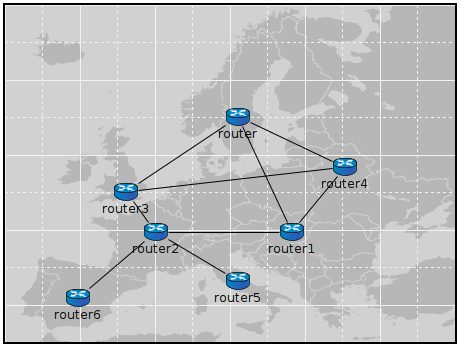
\includegraphics{figures/graphics-bgtags}
    \caption{Background grid, scaling and image}
    \label{fig:graphics-bgtags}
  \end{center}
\end{figure}

After specifying the above \ttt{bgs} tag, all your submodule coordinates will be treated as if
they were specified in km.

To see detailed descripton of the display string tags check
Appendix \ref{cha:display-string-tags} about display string tags.

\subsection{Connection display strings}

Connections may also have display strings. Connections inherit the
display string property of their channel in the same way submodules inherit
their display string from their types. If no channel is specified for a
connection, \cclass{IdealChannel} will be used implicitly by the simulation kernel.

Connections support the following tags:
\begin{itemize}
  \item{\ttt{ls} -- line shape, and colors}
  \item{\ttt{t} -- text}
  \item{\ttt{tt} -- tooltip}
  \item{\ttt{m} -- used for hinting Tkenv how the connections should route to/from the module}
\end{itemize}

Example of a thick, red connection:
\begin{verbatim}
source1.out --> { @display("ls=red,3"); } --> queue1.in++;
\end{verbatim}

\begin{center}
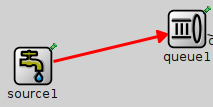
\includegraphics{figures/graphics-lstag}
\end{center}

\begin{note}
If you want to hide a connection, specify width=0 for the connection. i.e. use \ttt{ls=,0}.
\end{note}

To see detailed descripton of these tags check
Appendix \ref{cha:display-string-tags} about display string tags.

\subsection{Message display strings}

Message display string affects how messages are shown during animation.
By default, they are displayed as a small filled circle, in one of
8 basic colors (the color is determined as \textit{message kind modulo 8}),
and with the message class and/or name displayed under it
The latter is configurable in the Tkenv Options dialog, and message kind
dependent coloring can also be turned off there.

\subsubsection{Specifying message display strings}
Message objects do not store a display string by default, but you can redefine
the \cclass{cMessage}'s \ffunc{getDisplayString()} method and make it return
one.

Example of using an icon to represent a message:
\begin{verbatim}
const char *CustomPacket::getDisplayString() const
{
    return "i=msg/packet;is=vs";
}
\end{verbatim}

Or better: If you add the field \ffunc{displayString} to your message
definition (.msg file) the message compiler will automatically generate
the \ffunc{set/getDisplayString} methods for you:

\begin{verbatim}
message Job
{
    string displayString = "i=msg/package_s,kind";
...
\end{verbatim}

\subsubsection{Message display string tags}

The following tags can be used in message display strings:
\begin{itemize}
  \item{\ttt{b} -- shapes, colors}
  \item{\ttt{i} -- icon}
  \item{\ttt{is} -- icon size}
\end{itemize}

Using a small red box icon to represent the messages:
\begin{verbatim}
@display("i=msd/box,red;is=s");
\end{verbatim}

Messages will be represented by a 15x15 rectangle with white background.
Their border color will depend on the \ttt{messageKind} property of the message.
\begin{verbatim}
@display("b=15,15,rect,white,kind,5");
\end{verbatim}

\begin{note}
   In message display strings you may use the word \ttt{kind} as a special color.
   This virtual color depends on the \ttt{messageKind} field in the message.
\end{note}

%FIXME more examples, WITH EXPLANATIONS


\section{Parameter substitution}

Parameters of the module or channel containing the
display string can be substituted into the display string
with the \ttt{\$parameterName} notation:

Example:
\begin{verbatim}
simple MobileNode
{
    parameters:
        double xpos;
        double ypos;
        string fillColor;
        // get the values from the module parameters xpos,ypos,fillcolor
        @display("p=$xpos,$ypos;b=60,10,rect,$fillColor,black,2");
}
\end{verbatim}

\section{Colors}
\label{sec:ch-graphics:colors}

\subsection{Color names}

Any valid Tk color specification is accepted: English color names
(blue, lightgrey, wheat) or \textit{\#rgb}, \textit{\#rrggbb} format
(where \textit{r},\textit{g},\textit{b} are hex digits).

It is also possible to specify colors in HSB (hue-saturation-brightness) as
\textit{@hhssbb} (with \textit{h}, \textit{s}, \textit{b} being hex digits).
HSB makes it easier to scale colors e.g. from white to bright red.

You can produce a transparent background by specifying a hyphen (\textit{"-"})
as background color.

In message display strings, \ttt{kind} can also be used as a special color name.
It will map to a color depending on the message kind.
(See the \ffunc{getKind()} method of \cclass{cMessage}.)

\subsection{Icon colorization}

The \ttt{"i="} display string tag allows for colorization of icons.
It accepts a target color and a percentage as the degree of colorization.
Percentage has no effect if the target color is missing.
Brightness of icon is also affected -- to keep the original brightness,
specify a color with about 50\% brightness (e.g. \#808080 mid-grey,
\#008000 mid-green).

Examples:

\begin{itemize}
  \item \ttt{"i=device/server,gold"} creates a gold server icon
  \item \ttt{"i=misc/globe,\#808080,100"} makes the icon greyscale
  \item \ttt{"i=block/queue,white,100"} yields a "burnt-in" black-and-white icon
\end{itemize}

Colorization works with both submodule and message icons.


\section{The icons}
\label{sec:ch-graphics:icon-library}

\subsection{The image path}

In the current {\opp} version, module icons are PNG or GIF files. The icons shipped
with {\opp} are in the \ttt{images/} subdirectory. Both the graphical NED editor
and Tkenv need the exact location of this directory to load the icons.

Icons are loaded from all directories in the \textit{image path},
a semicolon-separated list of directories.
The default image path is compiled into Tkenv with the value
\ttt{"\textit{omnetpp-dir}/images; ./images;./bitmaps"} -- which will work fine
as long as you don't move the directory, and you'll also be able to
load more icons from the \ttt{images/} subdirectory of the current
directory. As people usually run simulation models from the model's
directory, this practically means that custom icons placed in the
\ttt{images/} subdirectory of the model's directory are automatically
loaded.

The compiled-in image path can be overridden with the \ttt{OMNETPP\_IMAGE\_PATH}
environment variable. The way of setting environment variables is system
specific: in Unix, if you're using the bash shell, adding a line

\begin{verbatim}
export OMNETPP_IMAGE_PATH="/home/you/images;./images"
\end{verbatim}

to \ttt{~/.bashrc} or \ttt{~/.bash\_profile} will do; on Windows, environment variables
can be set via the \textit{My Computer --> Properties} dialog.

You can extend the image path from \ffilename{omnetpp.ini} with the
\ttt{tkenv-image-path} option, which gets prepended to the environment
variable's value.

\begin{verbatim}
[General]
tkenv-image-path = "/home/you/model-framework/images;/home/you/extra-images"
\end{verbatim}


\subsection{Categorized icons}

Since {\opp} 3.0, icons are organized into several categories, represented
by folders. These categories include:

\begin{itemize}
  \item block/ - icons for subcomponents (queues, protocols, etc).
  \item device/ - network devices: servers, hosts, routers, etc.
  \item abstract/ - symbolic icons for various devices
  \item misc/ - node, subnet, cloud, building, town, city, etc.
  \item msg/ - icons that can be used for messages
\end{itemize}

Old (pre-3.0) icons are in the \ttt{old/} folder.

Tkenv and the IDE now load icons from subdirectories of all directories
of the image path, and these icons can be referenced from display strings
by naming the subdirectory (subdirectories) as well:
\ttt{"subdir/icon"}, \ttt{"subdir/subdir2/icon"}, etc.

For compatibility, if the display string contains a icon without
a category (i.e. subdirectory) name, {\opp} tries it as "old/icon" as well.

\subsection{Icon size}

Icons come in various sizes: normal, large, small, very small. Sizes are
encoded into the icon name's suffix: \ttt{\_vl}, \ttt{\_l}, \ttt{\_s}, \ttt{\_vs}.
In display strings, one can either use the suffix (\ttt{"i=device/router\_l"}),
or the \ttt{"is}" (\textit{icon size}) display string tag (\ttt{"i=device/router;is=l"}),
but not both at the same time (we recommend using the \ttt{is} tag whenever possible).


\section{Layouting}
\label{sec:ch-graphics:layouting}

{\opp} implements an automatic layouting feature, using
a variation of the SpringEmbedder algorithm. Modules which have
not been assigned explicit positions via the \ttt{"p="} tag will be
automatically placed by the algorithm.

SpringEmbedder is a graph layouting algorithm based on a physical model.
Graph nodes (modules) repent each other like electric charges
of the same sign, and connections are sort of springs which try
to contract and pull the nodes they're attached to. There is also friction
built in, in order to prevent oscillation of the nodes. The layouting algorithm
simulates this physical system until it reaches equilibrium
(or times out). The physical rules above have been slightly tweaked
to get better results.

The algorithm doesn't move any module which has fixed coordinates.
Predefined row, matrix, ring or other arrangements (defined
via the 3rd and further args of the \ttt{"p="} tag) will be preserved --
you can think about them as if those modules were attached
to a wooden framework so that they can only move as one unit.

Caveats:

\begin{itemize}
  \item If the full graph is too big after layouting, it is scaled
    back so that it fits on the screen, \textit{unless it contains
    any fixed-position module}. (For obvious reasons: if there's a module
    with manually specified position, we don't want to move that one).
    To prevent rescaling, you can specify a sufficiently large bounding
    box in the background display string, e.g. \ttt{"b=2000,3000"}.
  \item Size is ignored by the present layouter, so longish modules
    (such as an Ethernet segment) may produce funny results.
  \item The algorithm is prone to produce erratic results, especially
    when the number of submodules is small, or when using predefined
    (matrix, row, ring, etc) layouts. The "Re-layout" toobar button
    can then be very useful. Larger networks usually produce
    satisfactory results.
  \item The algorithm is starting from random positions.
     To get the best results you may experiment with
    different seeds by specifying them using the \ttt{bgl=\textit{seed}}
    display string tag.
\end{itemize}

\section{Enhancing animation}

\subsection{Changing display strings at runtime}

Often it is useful to manipulate the display string at runtime.
Changing colors, icon, or text may convey status change, and
changing a module's position is useful when simulating mobile
networks.

Display strings are stored in \cclass{cDisplayString} objects inside
channels, modules and gates. \cclass{cDisplayString} also lets you
manipulate the string.

To get a pointer to the \cclass{cDisplayString} object, you can call
the components's \ffunc{getDisplayString()} method:

\begin{verbatim}
// Setting a module's position, icon and status icon:
cDisplayString *dispStr = getDisplayString();
dispStr->parse("p=40,20;i=device/cellphone;i2=status/disconnect");
\end{verbatim}

\begin{note}
The connection display string is stored in the channel object, but it
can also be accessed via the source gate of the connection.
\end{note}

\begin{verbatim}
// Setting an outgoing connection's color to red:
cDisplayString *gateDispStr = gate("out")->getDisplayString();
dispStr->parse("ls=red");
\end{verbatim}

\begin{note}
In {\opp} 3.x, to manipulate the appearance of a compound module you had to use
the \ffunc{backgroundDisplayString()} method. This method is no longer
supported in {\opp} 4.0, because there is no separate background display string.
Use the \ffunc{getDisplayString()} method instead with the background
specific tags, i.e. those starting with \ttt{bg}.
\end{note}

\begin{verbatim}
// Setting module background and grid with background display string tags:
cDisplayString *parentDispStr = getParentModule()->getDisplayString();
parentDispStr->parse("bgi=maps/europe;bgg=100,2");
\end{verbatim}

As far as \cclass{cDisplayString} is concerned, a display string
(e.g. \ttt{"p=100,125;i=cloud"}) is a string that consist of several
\textit{tags} separated by semicolons, and each tag has a \textit{name}
and after an equal sign, zero or more \textit{arguments} separated by commas.

The class facilitates tasks such as finding out what tags a display string
has, adding new tags, adding arguments to existing tags,
removing tags or replacing arguments. The internal storage method allows
very fast operation; it will generally be faster than direct string manipulation.
The class doesn't try to interpret the display string in any way, nor does
it know the meaning of the different tags; it merely parses the string
as data elements separated by semicolons, equal signs and commas.

An example:

\begin{verbatim}
dispStr->parse("a=1,2;p=alpha,,3");
dispStr->insertTag("x");
dispStr->setTagArg("x",0,"joe");
dispStr->setTagArg("x",2,"jim");
dispStr->setTagArg("p",0,"beta");
ev << dispStr->str();  // result: "x=joe,,jim;a=1,2;p=beta,,3"
\end{verbatim}

\subsection{Bubbles}

Modules can let the user know about important events (such as a node
going down or coming up) by displaying a bubble with a short message
("Going down", "Coming up", etc.) This is done by the \ffunc{bubble()} method
of \cclass{cComponent}. The method takes the string to be displayed
as a \ttt{const char *} pointer.

An example:
\begin{verbatim}
bubble("Collision! (2 frames)");
\end{verbatim}
\begin{center}
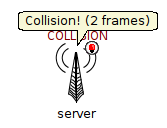
\includegraphics{figures/graphics-bubble}
\end{center}

If the module contains a lot of code that modifies the display string or
displays bubbles, it is recommended to make these calls conditional
on \ttt{ev.isGUI()}. The \ttt{ev.isGUI()} call returns \textit{false}
when the simulation is run under Cmdenv, so one can make the code skip
potentially expensive display string manipulation.

Better:
\begin{verbatim}
if (ev.isGUI())
    bubble("Going down!");
\end{verbatim}

%%% Local Variables:
%%% mode: latex
%%% TeX-master: "usman"
%%% End:
